\section{Single speaker source}
This section aims to introduce and analyse the fundamental for a single source, by analyse the behaviour of a piston source. The pressure around the piston source will be analysed analytically, to determine the radiation of a single speaker from \SI{60}{\hertz} and upwards and compare it with the measurement from \autoref{ch:polar_response}. The \SI{60}{\hertz} lower limit enable the simulation to be validated by measurement in the AAU anechoic chamber and is a used lower limit for the low/mid driver in some line source array \citep{V-DOSC}.  The analyse shall end out with a approximated simulation model of the \gls{dut}.

\subsection{Pressure analysis around a single source}
To characterised the directions properties of an analytical model of the \gls{dut}, the source will be modulated in two dimension as one piston source. The analysis of a piston source in to dimension built on a thin piston source in three dimension where the z dimension is fixed. The piston lays flat down so i look like a line and have radius $a$. The piston source will be considered as many small sources, where the complete surface vibrate radially with speed

\begin{equation}
u = \text{\textit{{\LARGE u}}}_{0} \cdot exp(j \omega t)
\end{equation}

    \startexplain
    		\explain{$u$ is the complex speed of the line source }{\si{1}}
        \explain{$\text{\textit{{\LARGE u}}}_{0}$ is the Amplitude}{\si{1}}
        \explain{$j$ is the imaginary unit }{\si{1}}
        \explain{$\omega$ is the angular velocity }{\si{1}}
        \explain{$t$ is the time }{\si{1}}
    \stopexplain
    
Each small sources is treated as an unbaffled simple source with length $dx$ and the source strange can be modulated as following      

\begin{equation}
dQ = \text{\textit{{\LARGE u}}}_{0} 2 \pi a \cdot dx
\end{equation}

    \startexplain
    		\explain{$dQ$ is the simple source strange }{\si{1}}
        \explain{$\text{\textit{{\LARGE u}}}_{0}$ is the Amplitude}{\si{1}}
        \explain{$a$ is the radius for cylinder }{\si{1}}
        \explain{$dx$ is the length for the simple source }{\si{1}}
    \stopexplain    
 
The following \autoref{fig:continues_line_source} shows an example of the continues line source where one of the small source is showed with length $dx$. 

\begin{figure}[H]
	\centering
\begin{picture}(0,0)%
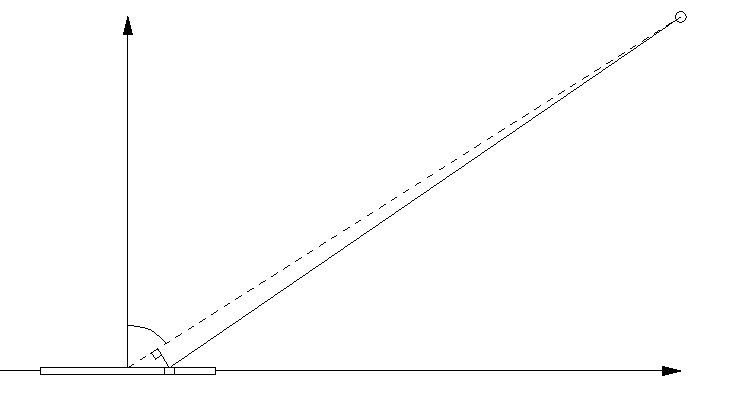
\includegraphics{line_source.pdf}%
\end{picture}%
\setlength{\unitlength}{746sp}%
%
\begingroup\makeatletter\ifx\SetFigFont\undefined%
\gdef\SetFigFont#1#2#3#4#5{%
  \reset@font\fontsize{#1}{#2pt}%
  \fontfamily{#3}\fontseries{#4}\fontshape{#5}%
  \selectfont}%
\fi\endgroup%
\begin{picture}(31223,16833)(-5411,-436)
\put(12106,7139){r'}%
\put(24121,15599){P(r,$\theta$,t)}%
\put(946,2684){$\theta$}%
\put(23851,659){x}%
\put(-89,16094){y}%
\put(11341,8354){r}%
\put(3466,-571){$a$}%
\put(1441,-376){ds}%
\put(-134,-421){0}%
\put(-4049,-571){$-a$}%
\put(226,1649){$\Delta$r}%
\end{picture}%
	\caption{The model of a continues line source (ref the book)}
		\label{fig:continues_line_source}
\end{figure}


\autoref{fig:continues_line_source} shows the concept with the 


\autoref{fig:single_speaker_model} shows the model of the speaker unit.







\begin{equation}
p(r,\theta ,t)=\frac{j}{2} \rho_{0}c  \text{\textit{{\LARGE u}}}_{0}\frac{a}{r}kL\left ( \frac{sin(\frac{1}{2}kLsin(\theta ))}{\frac{1}{2}kLsin(\theta )} \right )e^{j(\omega t-kr)}
\end{equation}
